% Options for packages loaded elsewhere
\PassOptionsToPackage{unicode}{hyperref}
\PassOptionsToPackage{hyphens}{url}
\PassOptionsToPackage{dvipsnames,svgnames,x11names}{xcolor}
%
\documentclass[
  letterpaper,
  DIV=11,
  numbers=noendperiod]{scrreprt}

\usepackage{amsmath,amssymb}
\usepackage{iftex}
\ifPDFTeX
  \usepackage[T1]{fontenc}
  \usepackage[utf8]{inputenc}
  \usepackage{textcomp} % provide euro and other symbols
\else % if luatex or xetex
  \usepackage{unicode-math}
  \defaultfontfeatures{Scale=MatchLowercase}
  \defaultfontfeatures[\rmfamily]{Ligatures=TeX,Scale=1}
\fi
\usepackage{lmodern}
\ifPDFTeX\else  
    % xetex/luatex font selection
\fi
% Use upquote if available, for straight quotes in verbatim environments
\IfFileExists{upquote.sty}{\usepackage{upquote}}{}
\IfFileExists{microtype.sty}{% use microtype if available
  \usepackage[]{microtype}
  \UseMicrotypeSet[protrusion]{basicmath} % disable protrusion for tt fonts
}{}
\makeatletter
\@ifundefined{KOMAClassName}{% if non-KOMA class
  \IfFileExists{parskip.sty}{%
    \usepackage{parskip}
  }{% else
    \setlength{\parindent}{0pt}
    \setlength{\parskip}{6pt plus 2pt minus 1pt}}
}{% if KOMA class
  \KOMAoptions{parskip=half}}
\makeatother
\usepackage{xcolor}
\setlength{\emergencystretch}{3em} % prevent overfull lines
\setcounter{secnumdepth}{5}
% Make \paragraph and \subparagraph free-standing
\makeatletter
\ifx\paragraph\undefined\else
  \let\oldparagraph\paragraph
  \renewcommand{\paragraph}{
    \@ifstar
      \xxxParagraphStar
      \xxxParagraphNoStar
  }
  \newcommand{\xxxParagraphStar}[1]{\oldparagraph*{#1}\mbox{}}
  \newcommand{\xxxParagraphNoStar}[1]{\oldparagraph{#1}\mbox{}}
\fi
\ifx\subparagraph\undefined\else
  \let\oldsubparagraph\subparagraph
  \renewcommand{\subparagraph}{
    \@ifstar
      \xxxSubParagraphStar
      \xxxSubParagraphNoStar
  }
  \newcommand{\xxxSubParagraphStar}[1]{\oldsubparagraph*{#1}\mbox{}}
  \newcommand{\xxxSubParagraphNoStar}[1]{\oldsubparagraph{#1}\mbox{}}
\fi
\makeatother


\providecommand{\tightlist}{%
  \setlength{\itemsep}{0pt}\setlength{\parskip}{0pt}}\usepackage{longtable,booktabs,array}
\usepackage{calc} % for calculating minipage widths
% Correct order of tables after \paragraph or \subparagraph
\usepackage{etoolbox}
\makeatletter
\patchcmd\longtable{\par}{\if@noskipsec\mbox{}\fi\par}{}{}
\makeatother
% Allow footnotes in longtable head/foot
\IfFileExists{footnotehyper.sty}{\usepackage{footnotehyper}}{\usepackage{footnote}}
\makesavenoteenv{longtable}
\usepackage{graphicx}
\makeatletter
\newsavebox\pandoc@box
\newcommand*\pandocbounded[1]{% scales image to fit in text height/width
  \sbox\pandoc@box{#1}%
  \Gscale@div\@tempa{\textheight}{\dimexpr\ht\pandoc@box+\dp\pandoc@box\relax}%
  \Gscale@div\@tempb{\linewidth}{\wd\pandoc@box}%
  \ifdim\@tempb\p@<\@tempa\p@\let\@tempa\@tempb\fi% select the smaller of both
  \ifdim\@tempa\p@<\p@\scalebox{\@tempa}{\usebox\pandoc@box}%
  \else\usebox{\pandoc@box}%
  \fi%
}
% Set default figure placement to htbp
\def\fps@figure{htbp}
\makeatother
% definitions for citeproc citations
\NewDocumentCommand\citeproctext{}{}
\NewDocumentCommand\citeproc{mm}{%
  \begingroup\def\citeproctext{#2}\cite{#1}\endgroup}
\makeatletter
 % allow citations to break across lines
 \let\@cite@ofmt\@firstofone
 % avoid brackets around text for \cite:
 \def\@biblabel#1{}
 \def\@cite#1#2{{#1\if@tempswa , #2\fi}}
\makeatother
\newlength{\cslhangindent}
\setlength{\cslhangindent}{1.5em}
\newlength{\csllabelwidth}
\setlength{\csllabelwidth}{3em}
\newenvironment{CSLReferences}[2] % #1 hanging-indent, #2 entry-spacing
 {\begin{list}{}{%
  \setlength{\itemindent}{0pt}
  \setlength{\leftmargin}{0pt}
  \setlength{\parsep}{0pt}
  % turn on hanging indent if param 1 is 1
  \ifodd #1
   \setlength{\leftmargin}{\cslhangindent}
   \setlength{\itemindent}{-1\cslhangindent}
  \fi
  % set entry spacing
  \setlength{\itemsep}{#2\baselineskip}}}
 {\end{list}}
\usepackage{calc}
\newcommand{\CSLBlock}[1]{\hfill\break\parbox[t]{\linewidth}{\strut\ignorespaces#1\strut}}
\newcommand{\CSLLeftMargin}[1]{\parbox[t]{\csllabelwidth}{\strut#1\strut}}
\newcommand{\CSLRightInline}[1]{\parbox[t]{\linewidth - \csllabelwidth}{\strut#1\strut}}
\newcommand{\CSLIndent}[1]{\hspace{\cslhangindent}#1}

\KOMAoption{captions}{tableheading}
\makeatletter
\@ifpackageloaded{bookmark}{}{\usepackage{bookmark}}
\makeatother
\makeatletter
\@ifpackageloaded{caption}{}{\usepackage{caption}}
\AtBeginDocument{%
\ifdefined\contentsname
  \renewcommand*\contentsname{Table of contents}
\else
  \newcommand\contentsname{Table of contents}
\fi
\ifdefined\listfigurename
  \renewcommand*\listfigurename{List of Figures}
\else
  \newcommand\listfigurename{List of Figures}
\fi
\ifdefined\listtablename
  \renewcommand*\listtablename{List of Tables}
\else
  \newcommand\listtablename{List of Tables}
\fi
\ifdefined\figurename
  \renewcommand*\figurename{Figure}
\else
  \newcommand\figurename{Figure}
\fi
\ifdefined\tablename
  \renewcommand*\tablename{Table}
\else
  \newcommand\tablename{Table}
\fi
}
\@ifpackageloaded{float}{}{\usepackage{float}}
\floatstyle{ruled}
\@ifundefined{c@chapter}{\newfloat{codelisting}{h}{lop}}{\newfloat{codelisting}{h}{lop}[chapter]}
\floatname{codelisting}{Listing}
\newcommand*\listoflistings{\listof{codelisting}{List of Listings}}
\makeatother
\makeatletter
\makeatother
\makeatletter
\@ifpackageloaded{caption}{}{\usepackage{caption}}
\@ifpackageloaded{subcaption}{}{\usepackage{subcaption}}
\makeatother

\usepackage{bookmark}

\IfFileExists{xurl.sty}{\usepackage{xurl}}{} % add URL line breaks if available
\urlstyle{same} % disable monospaced font for URLs
\hypersetup{
  pdfauthor={Adelson Guaraci Jantsch},
  colorlinks=true,
  linkcolor={blue},
  filecolor={Maroon},
  citecolor={Blue},
  urlcolor={Blue},
  pdfcreator={LaTeX via pandoc}}


\author{Adelson Guaraci Jantsch}
\date{}

\begin{document}

\renewcommand*\contentsname{Table of contents}
{
\hypersetup{linkcolor=}
\setcounter{tocdepth}{2}
\tableofcontents
}

\bookmarksetup{startatroot}

\chapter*{Meu caderno de notas}\label{meu-caderno-de-notas}
\addcontentsline{toc}{chapter}{Meu caderno de notas}

\markboth{Meu caderno de notas}{Meu caderno de notas}

\pandocbounded{
\includegraphics[keepaspectratio]{images/clipboard-3286838625.png}}

To learn more about Quarto books visit
\url{https://quarto.org/docs/books}.

\bookmarksetup{startatroot}

\chapter{Artes}\label{artes}

\section{Música}\label{muxfasica}

\href{https://bandcamp.com/}{Bandcamp}.

\href{https://www.epidemicsound.com/music/featured/?override_referrer=https\%3A\%2F\%2Fwww.epidemicsound.com\%2Foauth_callback\%2F&is_new_user=true}{Epidemic
Sound}. \#\# Fotografia

\href{https://juicyworld.org/alexander-gnatenko/}{Juicy World, Alexander
Gnatenko}.

\bookmarksetup{startatroot}

\chapter{Medicina Baseada em
Evidências}\label{medicina-baseada-em-eviduxeancias}

\href{https://deakin.libguides.com/ebp/process}{The 5 As of
evidence-based practice} - website desenvolvido pela Dunkin University.
This guide offers insights and resources for navigating the principles
and procedural steps of Evidence-Based Practice.

\section{Introdução}\label{introduuxe7uxe3o}

Nas semanas anteriores tivemos a oportunidade de revisar alguns
conceitos da epidemiologia clínica, como prevalência, incidência, risco
absoluto, risco relativo, redução absoluta do risco, número necessário a
tratar (NNT) e número necessário para causar dano (NNH).

Usamos alguns exemplos para ilustrá-los, bem como nos exercícios
propostos para a segunda semana. Mas se você prestou atenção, falamos
bastante sobre as dúvidas do Dr.~Josias ao atender a gestante Mariela.
Ele se perguntava sobre a eficácia do uso de aspirina e carbonato de
cálcio no seu caso. Estava em dúvida sobre qual era o real benefício do
uso destes medicamentos. Reformulamos suas dúvidas usando a estratégia
PICO da seguinte forma:

\begin{longtable}[]{@{}
  >{\raggedright\arraybackslash}p{(\linewidth - 0\tabcolsep) * \real{1.0000}}@{}}
\toprule\noalign{}
\endhead
\bottomrule\noalign{}
\endlastfoot
\textbf{P (paciente ou população):} gestante em risco de pré-eclâmpsia.
Há uma diferença aqui quanto à população - para cada uma delas, a
população muda um pouco. Para carbonato de cálcio, a população seria
``estar gestante'' e para aspirina a população passa a ser ``gestante em
risco de desenvolver pré-eclâmpsia. Vamos ver isto com detalhes mais
adiante. \\
\textbf{I (intervenção):} temos duas no momento -- (1) Aspirina e (2)
carbonato de Cálcio. \\
\textbf{C (Comparação)}: Nenhuma medicação ou uso de placebo. Para ambos
os casos, a intervenção seria fazer ou não-fazer. Não uma comparação
entre drogas distintas, com efeitos comparáveis. \\
\textbf{O (Outcome)}: ocorrência de pré-eclâmpsia -- e demais eventos
relacionados à pré-eclâmpsia que veremos adiante. \\
\end{longtable}

Se você já está dominando a estratégia PICO e aproveitou para abrir os
documentos e artigos das semanas passadas, já deve ter descoberto as
respostas para as dúvidas do Dr.~Josias. Se não é este o teu caso, não
se preocupe. Vamos fazer esta caminhada passo a passo até chegarmos às
respostas que queremos.

\begin{longtable}[]{@{}
  >{\raggedright\arraybackslash}p{(\linewidth - 0\tabcolsep) * \real{1.0022}}@{}}
\toprule\noalign{}
\endhead
\bottomrule\noalign{}
\endlastfoot
\emph{\texttt{ATENÇÃO:\ O\ caso\ da\ gestante\ Mariela\ não\ se\ resume\ à\ decisão\ de\ usar\ aspirina\ e\ carbonato\ de\ cálcio\ ou\ não.\ Sua\ vida,\ sua\ família,\ moradia\ e\ condições\ de\ vida,\ seu\ pré-natal,\ seu\ desejo\ ou\ não\ de\ ser\ mãe\ são\ maiores\ do\ que\ esta\ decisão\ e\ devem\ ser\ abordados\ pela\ equipe\ de\ saúde.\ Trabalhamos\ isso\ em\ diversos\ momentos\ do\ curso,\ buscando\ formar\ novos\ médicos\ que\ sabem\ olhar\ para\ o\ paciente\ e\ ver\ quem\ é\ a\ pessoa,\ sua\ doença\ e\ sua\ experiência\ de\ adoecimento.}}

\emph{\texttt{Hoje,\ seremos\ SMART!\ Lembram\ disso?\ Trataremos\ de\ um\ problema\ específico\ (S)\ e\ relevante\ (R)\ para\ a\ prática\ clínica,\ com\ uma\ atividade\ dimensionada\ (T)\ para\ que\ reforcem\ os\ conceitos\ deste\ ciclo\ ao\ final\ da\ leitura\ (A)\ e\ que\ consigam,\ ao\ menos,\ perceber\ que\ este\ assunto\ é\ mais\ fácil\ do\ que\ parece\ (M).}}

\emph{\texttt{Vamos\ nos\ aprofundar\ em\ um\ detalhe\ bem\ específico\ do\ cuidado\ pré-natal.\ Esta\ é\ uma\ oportunidade\ de\ mergulharmos\ fundo\ em\ um\ detalhe\ clínico\ que\ é\ percebido\ por\ muitos\ médicos\ como\ complicado\ demais.\ Medicina\ baseada\ em\ evidências\ não\ é,\ de\ forma\ alguma,\ mais\ importante\ do\ que\ possuirmos\ informações\ abrangentes\ sobre\ a\ paciente.\ Vamos\ apenas\ ser\ SMART\ e\ nos\ concentrar\ neste\ detalhe\ em\ específico\ por\ hoje.}} \\
\end{longtable}

\section{Fontes que apresentei nas semanas
anteriores:}\label{fontes-que-apresentei-nas-semanas-anteriores}

\href{https://bvsms.saude.gov.br/bvs/publicacoes/manual_gestacao_alto_risco.pdf}{Manual
de Gestação de Alto Risco do Ministério da Saúde}

\href{https://portaldeboaspraticas.iff.fiocruz.br/atencao-mulher/principais-questoes-sobre-profilaxia-da-pre-eclampsia-no-pre-natal/}{Principais
Questões sobre Profilaxia da pré-eclâmpsia no pré-natal}

Em
\href{https://www.gov.br/saude/pt-br/assuntos/noticias/2025/fevereiro/em-estrategia-contra-a-pre-eclampsia-suplementacao-de-calcio-passa-a-ser-universal-para-gestantes}{estratégia
contra a pré-eclâmpsia, suplementação de cálcio passa a ser universal
para gestantes} é a página do Ministério da Saúde apresentando esta
política nacional.

\href{https://www.gov.br/saude/pt-br/centrais-de-conteudo/publicacoes/notas-tecnicas/2024/nota-tecnica-conjunta-no-251-2024-coemm-cgesmu-dgci-saps-ms-e-cgan-deppros-saps-ms.pdf}{NOTA
TÉCNICA CONJUNTA Nº 251/2024-COEMM/CGESMU/DGCI/SAPS/MS E
CGAN/DEPPROS/SAPS/MS}

\href{https://obgyn.onlinelibrary.wiley.com/doi/epdf/10.1111/1471-0528.17222}{Calcium
for pre-eclampsia prevention: A systematic review and network
meta-analysis to guide personalised antenatal care}.

O artigo
\href{https://www.cfp.ca/content/cfp/70/1/38.full.pdf}{\emph{ASA use in
patients at risk of preeclampsia}}. apresenta um sumário de diversas
informações sobre o impacto da aspirina na ocorrência de pré-eclâmpsia.

\href{https://pmc.ncbi.nlm.nih.gov/articles/PMC6820858/}{Antiplatelet
agents for preventing pre-eclampsia and its complications}.

\href{https://www.who.int/publications/i/item/9789240003118}{WHO
recommendation on calcium supplementation before pregnancy for the
prevention of pre-eclampsia and its complications}.

\href{https://www.nejm.org/doi/10.1056/NEJMoa1704559?url_ver=Z39.88-2003&rfr_id=ori:rid:crossref.org&rfr_dat=cr_pub\%20\%200www.ncbi.nlm.nih.gov}{Aspirin
versus Placebo in Pregnancies at High Risk for Preterm Preeclampsia}.

Vamos começar respondendo a cada uma das perguntas PICO que elaboramos
anteriormente. Começando pela Aspirina.

\pandocbounded{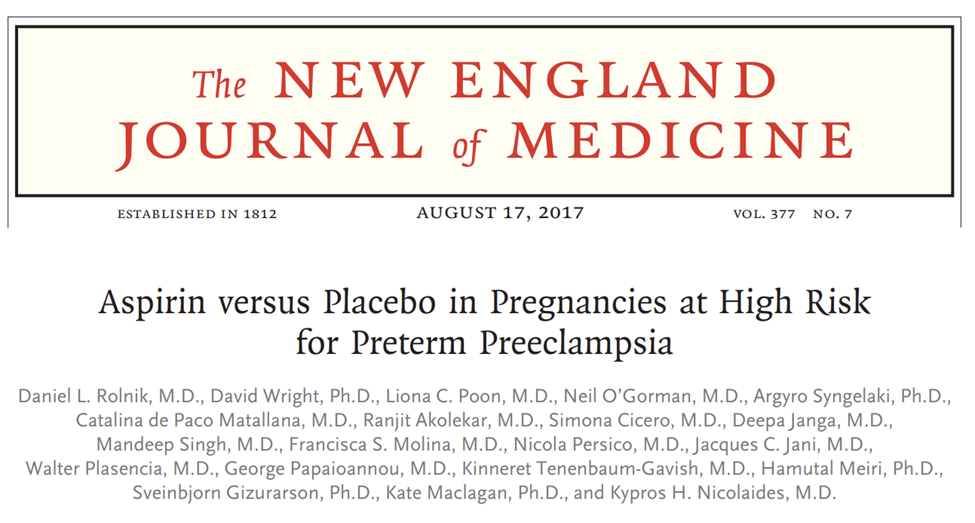
\includegraphics[keepaspectratio]{images/clipboard-4133286357.png}}

Neste artigo encontramos no resumo as seguintes informações:

\begin{longtable}[]{@{}
  >{\raggedright\arraybackslash}p{(\linewidth - 0\tabcolsep) * \real{1.0013}}@{}}
\toprule\noalign{}
\endhead
\bottomrule\noalign{}
\endlastfoot
\emph{In this multicenter, double-blind, placebo-controlled trial, we
randomly assigned 1776 women with singleton pregnancies who were at high
risk for preterm preeclampsia to receive aspirin, at a dose of 150 mg
per day, or placebo from 11 to 14 weeks of gestation until 36 weeks of
gestation. The primary outcome was delivery with preeclampsia before 37
weeks of gestation. The analysis was performed according to the
intention-to-treat principle.}

\emph{RESULTS A total of 152 women withdrew consent during the trial,
and 4 were lost to follow up, which left 798 participants in the aspirin
group and 822 in the placebo group. Preterm preeclampsia occurred in 13
participants (1.6\%) in the aspirin group, as compared with 35 (4.3\%)
in the placebo group (odds ratio in the aspirin group, 0.38; 95\%
confidence interval, 0.20 to 0.74; P=0.004). Results were materially
unchanged in a sensitivity analysis that took into account participants
who had withdrawn or were lost to follow-up. Adherence was good, with a
reported intake of 85\% or more of the required number of tablets in
79.9\% of the participants. There were no significant between-group
differences in the incidence of neonatal adverse outcomes or other
adverse events.}

\emph{CONCLUSIONS Treatment with low-dose aspirin in women at high risk
for preterm preeclampsia resulted in a lower incidence of this diagnosis
than placebo.} \\
\end{longtable}

Vamos traduzir para o português e entender o que está escrito ali:

Neste ensaio multicêntrico, duplo-cego, controlado por placebo,
\textbf{foram randomizadas 1776 mulheres com gestação única e alto risco
de pré-eclâmpsia prematura} para receber aspirina, na dose de 150 mg por
dia, ou placebo, de 11--14 semanas até 36 semanas de gestação. O
desfecho primário foi o parto por pré-eclâmpsia antes de 37 semanas de
gestação. A análise seguiu o princípio da intenção de tratar.

\textbf{Decifrando o que está escrito} -- 1776 mulheres em alto-risco de
pré-eclâmpsias, metade recebeu aspirina 150mg ao dia, a outra metade
recebeu placebo. Acompanharam ao longo da gestação e analisaram se
desenvolviam pré-eclâmpsia antes de 37 semanas de gestação.

\textbf{Detalhe:} Não precisa se preocupar com isto agora, mas se você
estiver se perguntando ``o que é intenção de tratar
(intention-to-treat)'', é uma forma de analisar os resultados
considerando todas as pacientes envolvidas no estudo desde o início.
Este método aproxima mais os resultados em direção do real efeito do
tratamento (efetividade do tratamento). É uma forma alternativa à
análise por protocolo (per protocolo analysis), que considera somente os
pacientes que concluíram o seguimento no estudo.

\textbf{RESULTADOS --} Um total de 152 mulheres retirou o consentimento
durante o estudo, e 4 foram perdidas ao seguimento, permanecendo 798
participantes no grupo aspirina e 822 no grupo placebo. A pré-eclâmpsia
prematura ocorreu em 13 participantes (1,6 \%) no grupo aspirina, em
comparação com 35 (4,3 \%) no grupo placebo (razão de chances {[}odds
ratio{]} no grupo aspirina, 0,38; intervalo de confiança de 95 \%,
0,20--0,74; P = 0,004). Os resultados mantiveram-se semelhantes em
análise de sensibilidade que considerou as participantes que desistiram
ou foram perdidas ao seguimento. A adesão foi satisfatória, com 79,9 \%
das participantes relatando ingestão de 85 \% ou mais dos comprimidos
prescritos. Não houve diferenças significativas entre os grupos quanto à
incidência de desfechos adversos neonatais ou outros eventos adversos.

\textbf{Decifrando o que está escrito} -- A razão de chances (uma forma
específica de risco relativo, não se preocupe com isso agora --
interprete esta informação como sendo o mesmo risco relativo que você já
conhece) foi de 0,38 e o intervalo de confiança variando entre 0,20 e
0,74. Este Risco Relativo de 0,38 é menor do que 1. Portanto, o risco de
pré-eclâmpsia com a intervenção (aspirina 150mg ao dia) é menor do que o
risco sem a aspirina -- quem recebeu placebo. Se fosse maior do que 1, a
aspirina aumentaria o risco de pré-eclâmpsia. Sobre a análise de
sensibilidade, não se preocupe com isso agora. Nada mais é do que um
escrutínio estatístico para se ter certeza de que o resultado encontrado
está correto. Terminam falando que as pacientes toleraram tomar aspirina
diariamente. ~

Dentro do artigo encontramos toda uma descrição minuciosa da metodologia
-- não se preocupe com isto hoje. E encontramos também uma tabela
apresentando os principais resultados encontrados. Ali encontramos que
13 mulheres que tomaram aspirina e 35 que receberam placebo,
desenvolveram pré-eclâmpsia. Em seguida descrevem os desfechos
secundários analisados no estudo (não é o que estamos observando hoje,
não se preocupe. Se concentre no desfecho primário (primary outcome),
pré-eclâmpsia antes de 37 semanas de gestação.

\pandocbounded{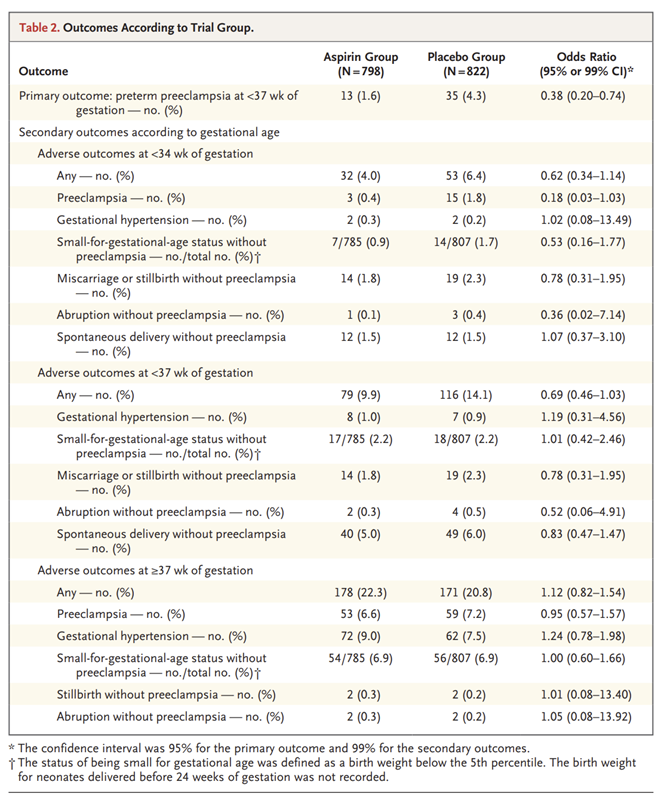
\includegraphics[keepaspectratio]{images/clipboard-3650889600.png}}

Vamos nos debruçar sobre estes números agora. Veja as imagens abaixo:

\pandocbounded{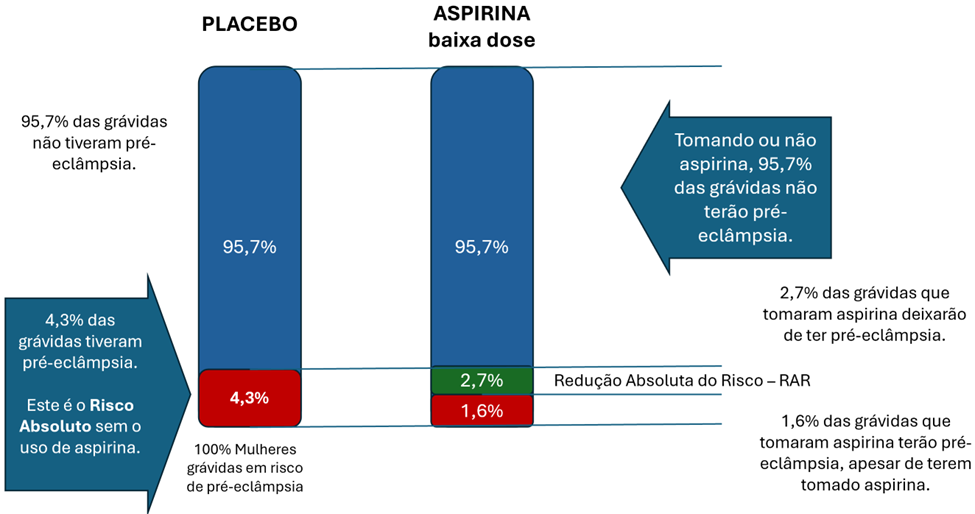
\includegraphics[keepaspectratio]{images/clipboard-3295726190.png}}

Em porcentagem, 95,7\% das mulheres em risco de desenvolver
pré-eclâmpsia não tiveram pré-eclâmpsia, mas 4,3\% tiveram. De onde
vieram estes números? Do grupo placebo, que se comporta como a população
normal, livre de intervenção. 4,3\% de incidência de pré-eclâmpsia está
próximo dos valores que encontramos naquele artigo brasileiro intitulado
\href{https://www.scielo.br/j/rbgo/a/qJLyYLLLvnfNC3d8hxJ68Lt/abstract/?lang=pt\#:~:text=A\%20frequ\%C3\%AAncia\%20acumulada\%20de\%20pr\%C3\%A9\%2Decl\%C3\%A2mpsia\%20foi\%20de,a\%20hipertens\%C3\%A3o\%20foi\%20de\%200\%2C5\%\%20a\%201\%2C7\%}{\textbf{Prevalência
de pré-eclâmpsia no Brasil: Uma revisão integrativa}} - 6,7\% para
pré-eclâmpsia, 1,7\% a 6,2\% para eclâmpsia e prematuridade associada a
hipertensão entre 0,5\% e 1,7\%.

Na segunda coluna temos que apenas 1,6\% das gestantes tiveram
pré-eclâmpsia no grupo que tomou aspirina. Isto nos leva a encontrar que
2,7\% das gestantes que usaram aspirina não tiveram pré-eclâmpsia. Estas
2,7\% de mulheres teriam pré-eclâmpsia, se não estivessem tomando
aspirina.

Mas e por que as mesmas 95,7\% das gestantes continuaram não tendo
pré-eclâmpsia? Porque não tiveram com o placebo e continuam não tendo
com a aspirina. Para estas mulheres, nem o placebo, nem a aspirina
fizeram diferença para elas, uma vez que não tinham e não terão
pré-eclâmpsia.

Resumindo, de todas as mulheres que usaram aspirina (100\% do braço
intervenção), apenas 2,7\% destas mulheres realmente se beneficiaram
desta medida preventiva. 97,3\% tomaram a aspirina em vão, sendo que
95,7\% destas não teriam pré-eclâmpsia de qualquer maneira e 1,6\% das
mulheres tiveram, mesmo tomando aspirina.

Isto nos leva à próxima imagem, onde calculamos que 37 mulheres em risco
de pré-eclâmpsia devem ganhar aspirina para que uma delas deixe de ter
pré-eclâmpsia.

\pandocbounded{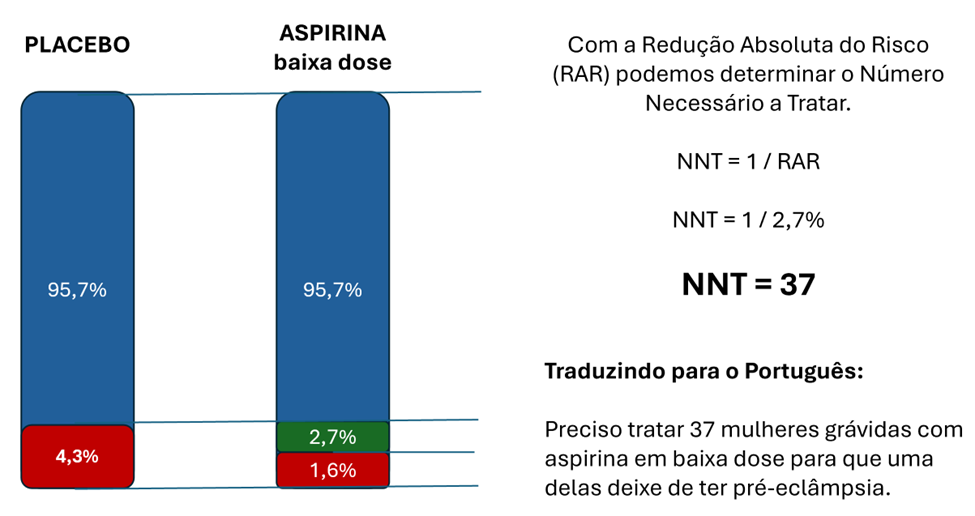
\includegraphics[keepaspectratio]{images/clipboard-3524595473.png}}

Se 37 tomaram aspirina e apenas 1 obteve o efeito desejado (evitar a
ocorrência de pré-eclâmpsia), 36 tomaram a medicação em vão. De forma
grosseira podemos dizer que 35 tomaram e não precisariam ter tomado,
pois não teriam pré-eclâmpsia de qualquer maneira, e 1 mulher (menos do
que uma, na verdade) tomou, mas teve pré-eclâmpsia mesmo assim.

Vamos ver se respondemos tudo o que queríamos?

\begin{longtable}[]{@{}
  >{\raggedright\arraybackslash}p{(\linewidth - 0\tabcolsep) * \real{0.9722}}@{}}
\toprule\noalign{}
\endhead
\bottomrule\noalign{}
\endlastfoot
\textbf{P (paciente ou população)}: gestantes em risco de pré-eclâmpsia.

\textbf{I (intervenção):} Aspirina

\textbf{C (Comparação)}: Nenhuma medicação ou uso de placebo.

\textbf{O (Outcome)}: ocorrência de pré-eclâmpsia. \\
\end{longtable}

Resumindo os passos e relembrando do PICO:

\begin{enumerate}
\def\labelenumi{\arabic{enumi}.}
\tightlist
\item
  Definimos qual a nossa população (\textbf{mulheres em risco de
  pré-eclâmpsia);}
\item
  Encontramos o risco absoluto nesta população -- esta medida veio do
  grupo controle que usou placebo (\textbf{Comparação});
\item
  Encontramos o risco no grupo que recebeu a intervenção (aspirina 150mg
  ao dia) (\textbf{Intervenção});
\item
  Encontramos o risco relativo, aqui chamado de odds ratio ou razão de
  chances.
\item
  Calculamos a redução absoluta do risco fazendo uma subtração simples
  do risco absoluto em quem recebeu placebo e o risco absoluto em quem
  recebeu aspirina (RAR = 4,3\% - 1,6\%) e encontramos 2,7\%. Ou seja, a
  redução absoluta do risco é igual a 2,7\%. Em português podemos dizer
  que reduzimos o risco de ocorrência de pré-eclâmpsia em 2,7\%,
  reduzindo de 4,3\% para 1,6\%. \textbf{(Outcome)}
\item
  Agora que conhecemos a nossa RAR (2,7\%), calculamos o NNT e
  encontramos que 37 mulheres em risco de pré-eclâmpsia devem tomar
  aspirina 150 mg ao dia para que uma destas mulheres deixe de ter este
  problema. \textbf{(Outcome)}
\end{enumerate}

Nenhuma conta complicada. Usamos apenas operações básicas que aprendemos
na escola -- subtração, porcentagem e regras de 3. Só isso.

E o carbonato de cálcio. Vamos seguir os mesmos passos. No artigo
\href{https://obgyn.onlinelibrary.wiley.com/doi/epdf/10.1111/1471-0528.17222}{Calcium
for pre-eclampsia prevention: A systematic review andnetwork
meta-analysis to guide personalised antenatal care} - uma revisão
sistemática e metanálise sobre o tema, encontramos o seguinte resumo:

\pandocbounded{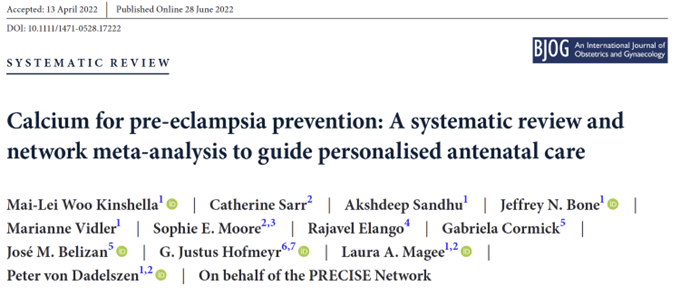
\includegraphics[keepaspectratio]{images/clipboard-3695179677.png}}

\pandocbounded{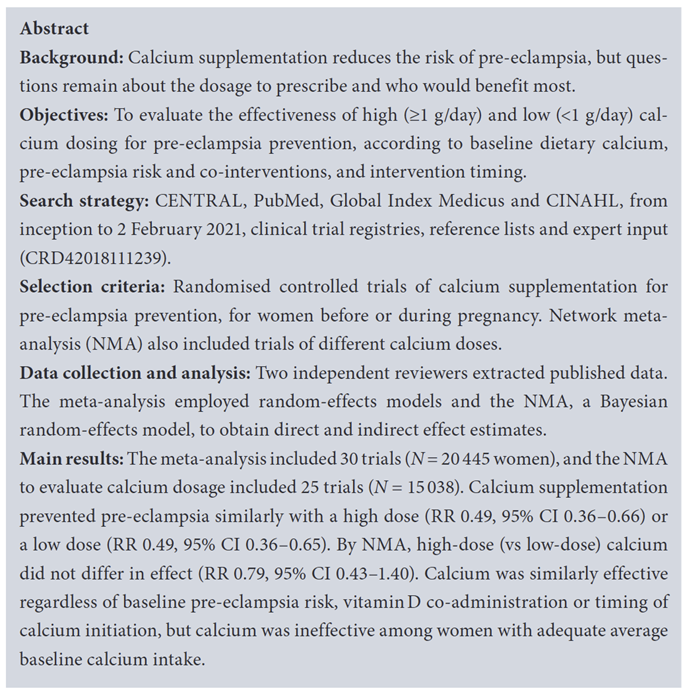
\includegraphics[keepaspectratio]{images/clipboard-4188042278.png}}

Em português e com comentários:

A suplementação de cálcio reduz o risco de pré-eclâmpsia, mas ainda há
dúvidas sobre a dosagem a prescrever e quais mulheres se beneficiam
mais. \textbf{Trata-se de uma revisão sistemática e metanálise sobre a
suplementação de cálcio como medida preventiva para ocorrência de
pré-eclâmpsia.}

\textbf{Objetivos:} Avaliar a eficácia de doses altas (≥ 1 g/dia) e
baixas (\textless{} 1 g/dia) de cálcio na prevenção da pré-eclâmpsia,
estratificando por ingestão dietética basal de cálcio, risco de
pré-eclâmpsia, co-intervenções e momento de início da suplementação.
\textbf{Aqui os autores descrevem todas as comparações que serão
analisadas.}

\textbf{Estratégia de busca:} Pesquisa nas bases CENTRAL, PubMed, Global
Index Medicus e CINAHL, desde a criação até 2 de fevereiro de 2021, além
de registros de ensaios clínicos, listas de referências e consulta a
especialistas (registro PROSPERO CRD42018111239).

\textbf{Critérios de seleção:} Ensaios clínico-randomizados de
suplementação de cálcio para prevenção de pré-eclâmpsia em mulheres
antes ou durante a gravidez. A análise em rede incluiu também ensaios
com diferentes dosagens de cálcio. \textbf{Aqui os autores descrevem
quais foram os tipos de estudos que entraram nas análises.}

\textbf{Coleta e análise de dados:} Dois revisores independentes
extraíram os dados publicados. A meta-análise empregou modelos de
efeitos aleatórios; a análise em rede utilizou modelo bayesiano de
efeitos aleatórios para estimativas de efeitos diretos e indiretos.

\textbf{Principais resultados:}

\begin{itemize}
\item
  Meta-análise com 30 ensaios (N = 20 445 mulheres) e análise em rede
  com 25 ensaios (N = 15 038).
\item
  A suplementação de cálcio preveniu pré-eclâmpsia de forma semelhante
  em altas doses (RR 0,49; IC 95\% 0,36--0,66) e baixas doses (RR 0,49;
  IC 95\% 0,36--0,65). \textbf{Não houve diferença no efeito entre alta
  e baixa dose.}
\item
  Pela análise em rede, não houve diferença entre dose alta e dose baixa
  (RR 0,79; IC 95\% 0,43--1,40).
\item
  O efeito foi consistente independentemente do risco basal de
  pré-eclâmpsia, da co-administração de vitamina D e do momento de
  início da suplementação.
\item
  Não houve benefício em mulheres com ingestão dietética média de cálcio
  considerada adequada.
\end{itemize}

Dentro do artigo encontramos a seguinte tabela, que nos mostra as
análises para altas doses de cálcio, baixas doses de cálcio e combinação
entre os dois grupos, ao final. Os resultados estão circulados em
vermelho.

\pandocbounded{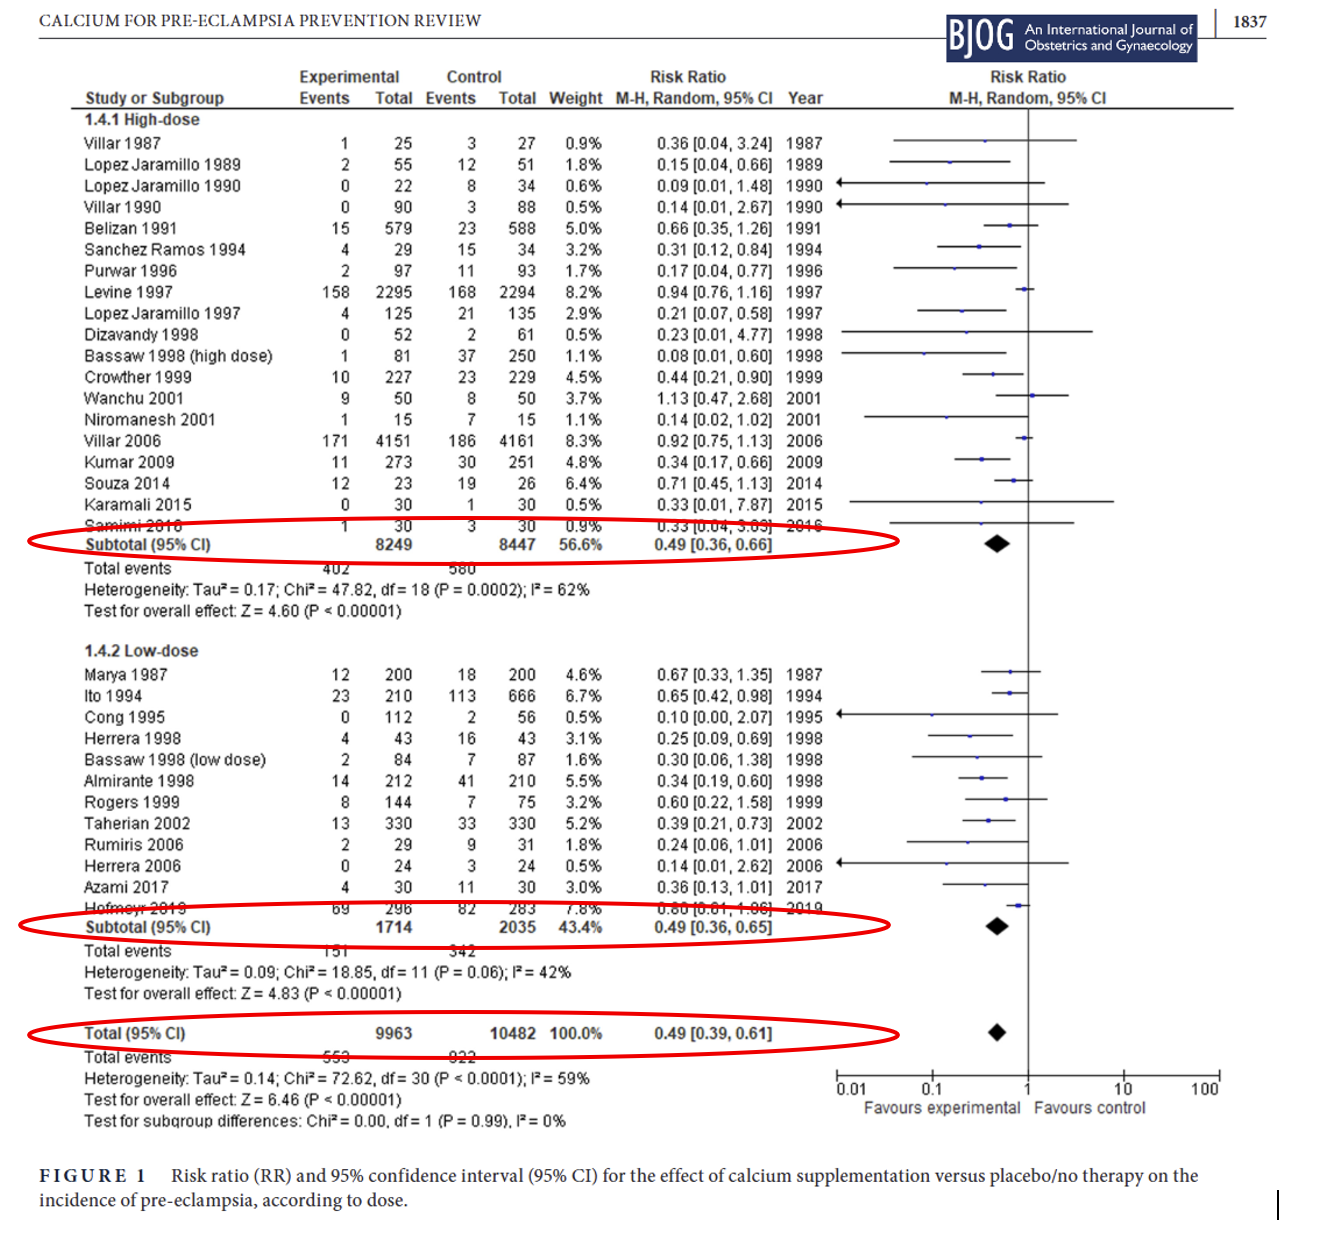
\includegraphics[keepaspectratio]{images/clipboard-3844703731.png}}

Vamos relembrar os passos que demos na nossa análise para a aspirina.

\begin{longtable}[]{@{}
  >{\raggedright\arraybackslash}p{(\linewidth - 0\tabcolsep) * \real{0.9722}}@{}}
\toprule\noalign{}
\endhead
\bottomrule\noalign{}
\endlastfoot
\textbf{P (paciente ou população)}: gestantes em risco de pré-eclâmpsia.

\textbf{I (intervenção):} carbonato de cálcio

\textbf{C (Comparação)}: Nenhuma medicação ou uso de placebo.

\textbf{O (Outcome)}: ocorrência de pré-eclâmpsia. \\
\end{longtable}

Resumindo os passos e relembrando do PICO:

1.~~~~~ Definimos qual a nossa população (\textbf{mulheres em risco de
pré-eclâmpsia);}

2.~~~~~ Encontramos o risco absoluto nesta população -- esta medida veio
do grupo controle que usou placebo (\textbf{Comparação}) --
\textbf{podemos usar a mesma medida do nosso estudo anterior e do artigo
brasileiro, com um valor entre 4 e 6\% das gestantes em risco
desenvolvendo pré-eclâmpsia ao longo da gestação.}

3.~~~~~ Encontramos o risco no grupo que recebeu a intervenção
(carbonato de cálcio) (\textbf{Intervenção}) -- aqui teremos que fazer o
caminho inverso. Encontrar o risco absoluto em quem recebeu o carbonato
de cálcio a partir do risco relativo;

4.~~~~~ Encontramos o risco relativo -- Carbonato de cálcio alta dose
(RR 0,49; IC 95\% 0,36--0,66) e baixas doses (RR 0,49; IC 95\%
0,36--0,65). \textbf{Não houve diferença no efeito entre alta e baixa
dose.}

Agora vamos calcular o risco absoluto em quem usou \textbf{carbonato de
cálcio}. Partindo de um número inteiro (5\%), se temos um risco relativo
de 0,49 para altas e baixas doses, teremos que o Risco Absoluto em quem
usou carbonato de cálcio no valor de 2,5\%. Em outras palavras, não
usando Carbonato de Cálcio o risco absoluto de pré-eclâmpsia é de 5\%.
Usando Carbonato de Cálcio o risco absoluto para pré-eclâmpsia reduz
para 2,5\%. Agora podemos calcular a \textbf{Redução Absoluta do Risco}.

5.~~~~~ Calculamos a \textbf{Redução Absoluta do Risco} fazendo uma
subtração simples do risco absoluto em quem recebeu placebo e o risco
absoluto em quem recebeu carbonato de cálcio (RAR = 5,0\% - 2,5\%) e
encontramos 2,5\%. Ou seja, a redução absoluta do risco é igual a 2,5\%.
Em português podemos dizer que reduzimos o risco de ocorrência de
pré-eclâmpsia em 2,5\%, reduzindo de 5,0\% para 2,5\%.
\textbf{(Outcome)}

6.~~~~~ Agora que conhecemos a nossa RAR (2,5\%), calculamos o NNT e
encontramos que 40 mulheres em risco de pré-eclâmpsia devem tomar
carbonato de cálcio para que uma destas mulheres deixe de ter este
problema. \textbf{(Outcome)}

\pandocbounded{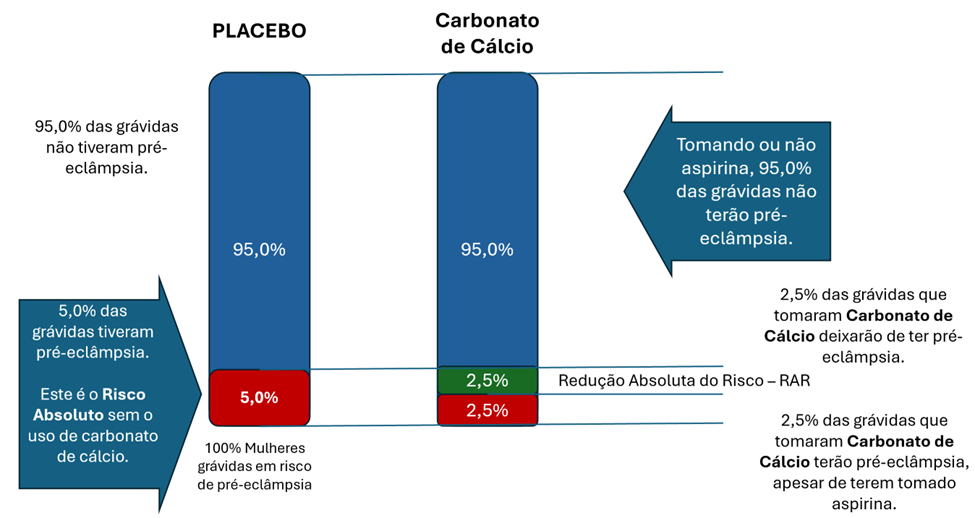
\includegraphics[keepaspectratio]{images/clipboard-2944778357.png}}

\pandocbounded{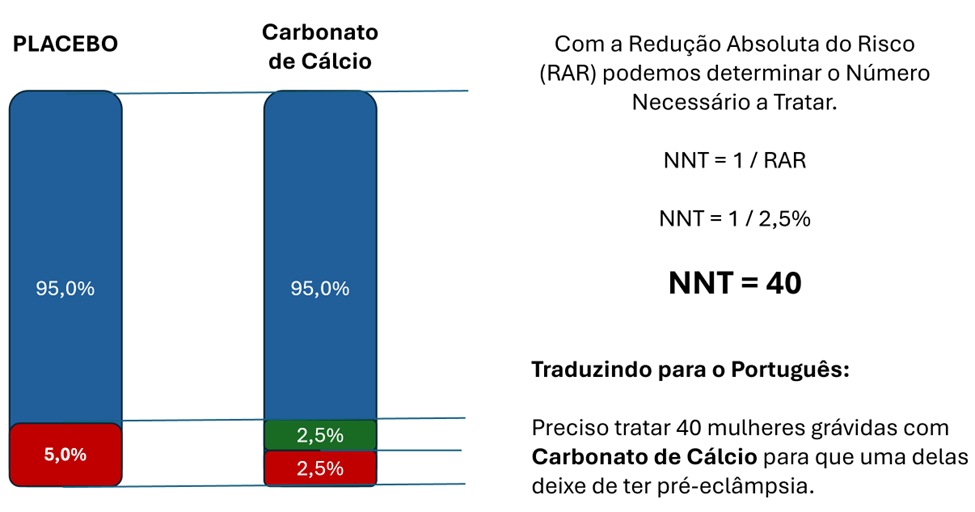
\includegraphics[keepaspectratio]{images/clipboard-1635376182.png}}

Frente a esta situação, Dr.~Josias pode ficar mais tranquilo de saber
que tanto a Aspirina quanto a suplementação com carbonato de cálcio
produzem benefícios consideráveis para prevenção de pré-eclâmpsia em
gestantes. No caso da sua paciente, a gestante Mariela, que tinha
medidas de pressão arterial elevadas previamente à gestação, pode ser
considerada como hipertensão arterial prévia a gestação -- um fator de
risco para pré-eclâmpsia. Com isto, devemos começar tanto a aspirina em
baixas doses quanto a suplementação de cálcio. Contudo, ele não começou
estas medicações somente por que o protocolo ministerial orienta, mas
sim por que, em concordância com as recomendações ministeriais e baseado
em boas evidências científicas, sabe agora que o risco absoluto de
pré-eclâmpsia para Mariela pode se reduzir em torno de 50\% a 65\% e que
ao prescrever aspirina e carbonato de cálcio para 30 a 40 mulheres
grávidas com perfil semelhante ao de Mariela, ao menos uma deixará de
desenvolver pré-eclâmpsia e terá um final de gestação com menos eventos
adversos.

Em tempo -- este parágrafo acima é uma generalização. Não tome os
valores ao pé da letra, pois não podemos afirmar com certeza que Mariela
será a pessoa que se beneficiará destas medidas preventivas.

\begin{longtable}[]{@{}
  >{\raggedright\arraybackslash}p{(\linewidth - 0\tabcolsep) * \real{1.0025}}@{}}
\toprule\noalign{}
\endhead
\bottomrule\noalign{}
\endlastfoot
\emph{\texttt{Mais\ um\ detalhe\ sobre\ a\ gestante\ Mariela.\ Falamos\ no\ começo\ deste\ documento\ que\ a\ gestante\ Mariela,\ sua\ vida,\ sua\ família\ e\ sua\ gestação\ era\ muito\ mais\ do\ que\ uma\ única\ decisão\ –\ fazer\ ou\ não\ aspirina\ e\ carbonato\ de\ cálcio.}}

\emph{\texttt{Foi\ importante\ lembrar\ disso\ no\ começo.\ Agora,\ nesta\ última\ página,\ acredito\ que\ vocês\ se\ sintam\ mais\ capazes\ de\ encarar\ discussões\ sobre\ medicina\ baseada\ em\ evidências.\ Aos\ poucos,\ vamos\ aprendendo\ a\ combinar\ estas\ habilidades\ com\ o\ método\ clínico\ centrado\ na\ pessoa\ e\ tudo\ aquilo\ que\ aprendemos\ sobre\ saber\ olhar\ para\ o\ paciente,\ ver\ quem\ é\ a\ pessoa,\ sua\ doença,\ sua\ experiência\ de\ adoecimento.}} \\
\end{longtable}

Qual a diferença entre fazer todo este percurso que fizemos nestas
semanas e simplesmente seguir o protocolo recomendado pelo Ministério da
Saúde? Pode até parecer que foi um trabalho desnecessário, mas agora
vocês conhecem um pouco mais o que está dentro desta caixa-preta, como
funcionam as comparações e as estatísticas por trás de uma recomendação
profilática como esta.

Por ora, todos vocês precisam se apropriar cada vez mais destes
princípios da Prática Clínica Baseada em Evidências. Isto tornará a
prática de todos trará.

Possivelmente muitos de vocês ocuparão cargos de gestão em diversos
níveis no futuro. Ter domínio destas ferramentas é fundamental para
poder \textbf{pautar decisões e desenhar políticas baseadas em
evidências.}

\bookmarksetup{startatroot}

\chapter{Consultancies in International
Health}\label{consultancies-in-international-health}

\section{Jobs}\label{jobs}

\href{https://www.unjobnet.org/}{UNJOBNET}. All jobs in one platform.
Access the complete list of job openings in all the United Nations and
major international organizations. More opportunities. Less search.

\href{https://globalhealthjobs.com/}{Global Health Jobs}. Over 250,000
global health professionals trust us to find verified jobs from top
NGOs, public health bodies, and humanitarian groups. Your next impactful
role starts here.

\href{https://www.pih.org/}{Partners in Health}

APPLYING FOR UNFPA JOBS -
\href{https://www.unfpa.org/sites/default/files/resource-pdf/Quantum\%20-\%20External\%20Application\%20Guide\%20August\%202022\%20.pdf}{STEP-BY-STEP
GUIDE}

\href{https://www.rockefellerfoundation.org/}{Rockfeller Foundation}. A
Rockefeller Foundation é uma organização filantrópica global que tem
como propósito promover o bem-estar da humanidade por meio de parcerias
estratégicas e financiamentos orientados a resultados; atua
principalmente em saúde pública, segurança alimentar, energia limpa e
mudanças climáticas, inclusão financeira e inovação social, oferecendo
subsídios a pesquisas e projetos, reunindo diferentes setores em fóruns
colaborativos, apoiando pilotos e modelos replicáveis, e influenciando
políticas públicas para gerar impactos sustentáveis e equitativos em
todo o mundo.

\href{https://cfpsdata.pku.edu.cn/\#/home}{CFPS - China Family Panel
Studies}.

\href{https://pedaids.org/}{he Elizabeth Glaser Pediatric AIDS
Foundation}. Founded over 30 years ago, The Elizabeth Glaser Pediatric
AIDS Foundation is committed to a comprehensive response to fighting HIV
and AIDS through research, global advocacy, strengthening of local
health care systems, and growing the capacity of governments and
communities in the world's most affected regions to respond to urgent
needs.

\href{https://www.vitalstrategies.org/about-us/business-and-consulting-opportunities/}{Vital
Strategies} strives to purchase high-quality goods and services at the
best value in a timely and transparent manner, which includes the
publication of all solicitations.

\href{https://jobs.unicef.org/en-us/listing/?jobnotfound=true}{UNICEF}.

The
\href{https://www.clintonhealthaccess.org/about-us/\#history}{Clinton
Health Access Initiative} (CHAI) is a global health organization that
operates at the nexus of government, business, and health. Our approach
hinges on our trusted relationships with governments to drive change
across entire health systems.

\href{https://www.villagereach.org/}{VillageReach} transforms health
care delivery to reach everyone.

At \href{https://www.gopa.de/\#jump-list-target-191-0}{GOPA Worldwide
Consultants}, we understand that behind each development project there
is a human story. For this reason, we favour dynamic development
cooperation that places beneficiaries at the heart of our work.

At \href{https://www.developmentaid.org/}{DevelopmentAid} we are
familiar with the challenges you encounter in the development sector.
Whether you're searching for funding opportunities, partners and experts
or interested in securing a job in the sector, we are ready to provide
you with the most innovative business intelligence and career aid tools
to assist you at every step of your way.

\href{https://www.evaplan.org/}{evaplan GmbH at the University Hospital
Heidelberg} is a consultancy company that undertakes advisory missions
and engages in implementation and accompanying research, project
implementation and capacity building in the field of international
health and social protection. Our mission is to help improve the health
of populations and individuals in Low \& Middle Income Countries (LMIC)
in the first place. Since more than 30 years we bridge the gap between
academic research and implementation striving to translate scientific
knowledge and technicity into practice.

\href{https://evaluation.org.uk/about-us/}{UK Evaluation Society}.
Through our work, we connect people, build learning communities, provide
expert-led training, and advocate for the importance of evidence-based
evaluation. Our goal is to share best practice and create a safe
learning environment where everyone feels welcome, can contribute and be
heard.

The \href{https://www.adb.org/who-we-are}{Asian Development Bank} (ADB)
envisions a prosperous, inclusive, resilient, and sustainable Asia and
the Pacific, while sustaining its efforts to eradicate extreme poverty
in the region.

\href{https://thepalladiumgroup.com/areas-expertise/health}{Palladium}
strengthens local partners and communities to take a comprehensive and
multifaceted approach to improving primary health care.

\href{https://m4health.pro/about-us/}{management4health} was founded in
2012 as a partnership of health sector professionals specialized in the
design, the implementation and the monitoring and evaluation of
international health projects and programmes. Together with our
partners, we work towards a shared vision of universal health coverage-
accessible, affordable, appropriate health services for all- through
stronger health systems. We strive for growth and development in a
sustainable manner, with the aim of becoming a key stakeholder and
operator in international health.

\href{https://doctorswithafrica.org/}{Medici con l'Africa Cuamm}. Our
mission is to advocate the universal right to health and promote the
values of international solidarity, justice and peace. We work to
protect and improve the wellbeing and health of vulnerable communities
in Africa with a long-term development perspective.

\bookmarksetup{startatroot}

\chapter{Research tools and
Partnerships}\label{research-tools-and-partnerships}

\href{https://www.napcrg.org/}{NAPCRG} supports and nurtures clinicians,
scientists, students and patients around the world as they pursue
primary care research.

\href{https://www.adfm.org/programs/brc-fellowship/}{The Building
Research Capacity (BRC) Fellowship}.

\href{https://saude.prefeitura.rio/comite-de-etica-em-pesquisa/}{Comitê
de Ética em Pesquisa do Rio de Janeiro}.

\href{https://icphc.iphce.org/}{International Conference on Primary
Health Care - ICPHC 2025}.

\href{https://healthsystemsfacts.org/?_gl=1\%2A1aq2uve\%2A_up\%2AMQ..\%2A_ga\%2AMTUxMzYxNjc4OS4xNzUwNDcxMTI2\%2A_ga_SDY74B5S30\%2AczE3NTA0NzExMjQkbzEkZzAkdDE3NTA0NzExMjQkajYwJGwwJGgw}{World
Health Systems Facts} is a project of the~Real Reporting Foundation.

\href{https://www.path.org/what-we-do/}{PATH} advances scientific
research, engineers cutting-edge technologies, crafts evidence-based
policies, and scales up resources, tools, and systems that transform
lives.

\href{https://researchrabbitapp.com/}{Research Rabbit App} - Ferramenta
que facilita a busca de conexões entre artigos científicos.

\href{https://publichealth.jhu.edu/academics/implementation-science-and-research-practice-certificate-program}{Implementation
Science and Research Practice Certificate Program}. Implementation
Science is the study of methods to promote the adoption, integration,
and sustainment of evidence-based practices, interventions or policies
into practice.

\href{https://www.isglobal.org/en/about-us}{ISGlobal Barcelona Institute
for Global Health}. The Barcelona Institute for Global Health, ISGlobal,
is the fruit of an innovative alliance between the ``la Caixa''
Foundation, academic institutions and government bodies to contribute to
the efforts undertaken by the international community to address the
challenges in global health.

O \href{https://www.globalhealthlearning.org/pt/courses}{Global Health
eLearning Center} (Centro de eLearning de Saúde Global oferece cursos
destinados a aumentar os seus conhecimentos sobre diversas áreas
técnicas de saúde global. Segue-se uma lista completa dos cursos. Os
programas de certificação também incluem cursos individuais, indicados à
esquerda e na página do Programa de Certificação.

\href{https://globalhealthtrainingcentre.tghn.org/elearning/}{Global
Health Training Center}

\href{https://tdrmooc.org/login?next=/dashboard}{TDR for research on
diseases of poverty}. Plataforma de ensino da UNICEF, UNDP, World Bank e
WHO.

\href{https://research-and-innovation.ec.europa.eu/funding/funding-opportunities/funding-programmes-and-open-calls/horizon-europe/cluster-1-health_en}{European
Commission - Research and innovation}

The \href{https://implementation.eu/}{European Implementation
Collaborative} engages a broad range of individual and organisational
stakeholders in the field of implementation. We build links and exchange
learning about implementation science and practice within Europe.

\href{https://internationalhealth.charite.de/en/}{The postgraduate study
programme ``International Health''} is hosted by Institute of
International Health at Charité -- Universitäsmedizin Berlin and offers
a master's course and two diploma courses.

The \href{https://ecsahc.org/ecsa-hc-at-a-glance/}{East, Central and
Southern Africa Health Community} (ECSA-HC) is an inter-governmental
health organization that fosters and promotes regional cooperation in
health among member states. Member states of the ECSA Health Community
are Kenya, Lesotho, Malawi, Mauritius, Eswatini, United Republic of
Tanzania, Uganda, Zambia and Zimbabwe.

\href{https://www.globalfamilymed.org/}{Global Familymed Foundation}
supports Family Medicine training where access to quality health care is
limited. Family Medicine graduates provide primary health care, which
addresses the main health problems in the community; providing
preventive, curative and rehabilitative services. We bring quality,
holistic health care to those who need it the most.

\section{Funding}\label{funding}

\href{https://wellcome.org/research-funding}{Welcome.org} - We fund
research to improve life, health and wellbeing through new knowledge and
understanding.

The \href{https://www.globalhealth.de/about/}{German Alliance for Global
Health Research} (GLOHRA) is an association of researchers from public
research institutions in Germany. We are committed to tackling today's
global health challenges via interdisciplinary and collaborative global
health research.

\href{https://dff.dk/en/apply-for-funding/}{Independent Research Fund
Denmark} - Apply for research funding and get support for your
application.

\href{https://novonordiskfonden.dk/en/}{Novo Nordisk Foundation} - We
are an independent, Danish enterprise foundation that supports
scientific, humanitarian and social causes.

\bookmarksetup{startatroot}

\chapter{Articles by topics}\label{articles-by-topics}

\section{My articles}\label{my-articles}

\href{https://rbmfc.org.br/rbmfc/article/view/2466/1565}{Scientific
research, primary care and family medicine: three essential ingredients
for improving the quality of health care} Rev Bras Med Fam Comunidade.
Rio de Janeiro, 2020 Jan-Dec; 15(42):24661.

\href{https://bmcprimcare.biomedcentral.com/articles/10.1186/s12875-021-01542-5}{Detection
and follow-up of chronic health conditions in Rio de Janeiro -- the
impact of residency training in family medicine}

\href{https://pmc.ncbi.nlm.nih.gov/articles/PMC8852675/pdf/bmjopen-2021-051515.pdf}{Residency
training in family medicine and its impact on coordination and
continuity of care: an analysis of referrals to secondary care in Rio de
Janeiro}

\href{https://journals.plos.org/globalpublichealth/article?id=10.1371/journal.pgph.0000547}{The
impact of residency training in family medicine on hospital admissions
due to Ambulatory-care Sensitive Conditions in Rio de Janeiro}

\section{Brazil, Primary Care and Primary Health
Care}\label{brazil-primary-care-and-primary-health-care}

\subsection{Multisectoral policies and
actions}\label{multisectoral-policies-and-actions}

\href{https://www.thelancet.com/journals/lanpub/article/PIIS2468-2667\%2825\%2900091-X/fulltext}{Health
effects of the Brazilian Conditional Cash Transfer programme over 20
years and projections to 2030: a retrospective analysis and modelling
study}

\section{Implementation Research}\label{implementation-research}

\href{https://pubmed.ncbi.nlm.nih.gov/32794412/}{Implementing Serious
Illness Communication Processes in Primary Care: A Qualitative Study}.
We conducted semi-structured interviews of participating primary care
physicians, nurse care coordinators, and social workers and coded
transcripts to assess the activities used to integrate Serious Illness
Care Program (SICP) into the workflow.

\bookmarksetup{startatroot}

\chapter*{References}\label{references}
\addcontentsline{toc}{chapter}{References}

\markboth{References}{References}

\phantomsection\label{refs}
\begin{CSLReferences}{0}{1}
\end{CSLReferences}




\end{document}
